\chapter{Introduction}
\section{Problem Statement}
%\indent{
\hspace*{0.82cm}Today smart phones are not exclusive property of early adopters or IT professionals.
Global Smart phone shipments grew a relatively healthy 43 per cent year-over-year to reach
600 million units in Q2 2010. According to comScore’s report, 234 million Americans
subscribed to mobile phone plans in January 2010. Of these 42.7 million owned internet
accessible smart phones, this represented an 18 per cent increase over the three months ended
in October.\\[0.5cm]
\hspace*{0.82cm}Important progress in mobile computing should start with straightforward local
convergence of Smartphones and computer infrastructure via simplistic mobile use model.
This use model would enhance the current synchronization schemes by by-passing the
synchronized data over proprietary services and giving the user the full control and full
accessibility of his/her own data both on the smart phone, as well on his very own
synchronization server. It is not always advisable for users to use synchronization services
provided by Google for android devices.\\[0.5cm]
\hspace*{0.82cm}These services may not ensure full privacy of all the data of the user. This data is
stored on the Google clouds. Also, today the security issues in cloud computing have not
been fully resolved. Hence it cannot be said our data remains fully secure when it is on
Google premises. Synchronization can be done by various means by the use of this product.
Offline and online mode synchronization is possible. Online mode can be used when user is
on-the-go and offline synchronization may be used when user is at the office or at home.\\[0.5cm]
%}
\section{Project Objective}
\hspace*{0.82cm}The project addresses the idea of android smartphones being synchronized in an
online and offline manner. A server application in the form of a desktop application and a
client application in the form of an android application is to be developed to achieve this
objective.\\[0.5cm]
The basic objectives of the project include:
\begin{itemize}
%\begin{spacing}{0}{
 \item Setting up a secure online connection of the mobile phone to the server.
 \item Setting up interfacing techniques to connect the mobile phones to the PC via a USB
cable, Bluetooth link or Wi-Fi.
 \item Devising a protocol which will control the authentication of the device, flow of data
in and out of the smartphone and the server.
 \item Managing user account on the server application.
 \item Developing the application such that it is cross-platform compatible i.e. it can be
deployed on a PC running any OS – Linux, Mac OSX or Windows.
%}\end{spacing}
\end{itemize}

\section{Architecture of the System}
\subsection{Current system}
\hspace*{0.82cm}The current system being used for synchronization involves the data being
synchronized to be synced via a Google account the user has to maintain. This means data
will have to be given to a third-party provider like Google when it actually not really
necessary to do so.\\[0.5cm]
This scenario is illustrated in figure 1.1.

\begin{figure}[H]
  \centering
    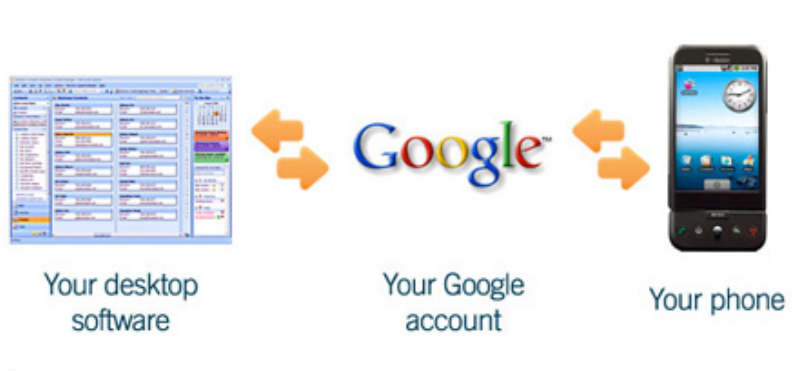
\includegraphics[height= 5cm, width=13cm]{project/images/architecture-current}
  \caption{\textbf{Architecture of Current System}}
\end{figure}

It is not always possible to store sensitive information on third-party premises 
like Google. This sensitive information can be in the form of phone logs, SMS, 
contacts, e-mails, notes, calendar schedules, etc.

\subsection{Proposed System}
\hspace*{0.82cm}The proposed system enables Android mobile device to be synchronized by the user
using this product such that all data may be synchronized in a private mutually exclusive
manner. This is illustrated in figure 1.2.

\begin{figure}[H]
  \centering
    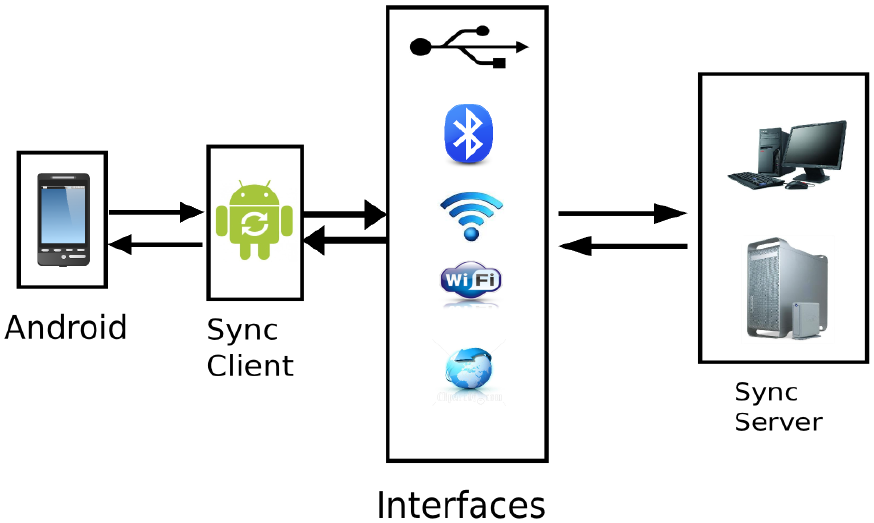
\includegraphics[height= 10cm, width=15cm]{project/images/architecture-proposed}
  \caption{\textbf{Architecture of Proposed System}}
\end{figure}

In this system, the android smartphone is connected to the server and after the
connections is established, synchronization may be started using any mode- offline or online
i.e. using a Cable or Wi-Fi or over a secure internet connection.
\newpage
\section{Licensing}
\subsection{GNU General Public License}
\hspace*{0.82cm}The GNU General Public License (GNU GPL or simply GPL) is the most widely used free software license, originally written by 
Richard Stallman for the GNU Project.\\[0.5cm]
\hspace*{0.82cm}The GPL is the first copyleft license for general use, which means that derived works can only be distributed under the 
same license terms. Under this philosophy, the GPL grants the recipients of a computer program the rights of the free software definition 
and uses copyleft to ensure the freedoms are preserved, even when the work is changed or added to. This is in distinction to permissive 
free software licenses, of which the BSD licenses are the standard examples.\\[0.5cm]
\hspace*{0.82cm}The text of the GPL is not itself under the GPL. The license's copyright disallows modification of the license. Copying 
and distributing the license is allowed since the GPL requires recipients to get "a copy of this License along with the Program".According 
to the GPL FAQ, anyone can make a new license using a modified version of the GPL as long as he or she uses a different name for the license, 
does not mention "GNU", and removes the preamble, though the preamble can be used in a modified license if permission to use it is obtained 
from the Free Software Foundation (FSF).\\[0.5cm]
\textbf{Version 2}\\
\hspace*{0.82cm}According to Richard Stallman, the major change in GPLv2 was the "Liberty or Death" clause, as he calls it — Section 7. 
This section says that if somebody has restrictions imposed that prevent him or her from distributing GPL-covered software in a way that 
respects other users' freedom (for example, if a legal ruling states that he or she can only distribute the software in binary form), he 
or she cannot distribute it at all. The hope is, that this will make it less tempting for companies to use patent threats to require a fee 
from the free software developers.\\[0.5cm]
\hspace*{0.82cm}By 1990, it was becoming apparent that a less restrictive license would be strategically useful for the C library and 
for software libraries that essentially did the job of existing proprietary ones; when version 2 of the GPL (GPLv2) was released in 
June 1991, therefore, a second license – the Library General Public License — was introduced at the same time and numbered with version 
2 to show that both were complementary. The version numbers diverged in 1999 when version 2.1 of the LGPL was released, which renamed it 
the GNU Lesser General Public License to reflect its place in the philosophy.\\[0.5cm]
\textbf{Terms and Conditions}\\
\hspace*{0.82cm}The terms and conditions of the GPL must be made available to anybody receiving a copy of the work that has a GPL applied to 
it ("the licensee"). Any licensee who adheres to the terms and conditions is given permission to modify the work, as well as to copy and 
redistribute the work or any derivative version. The licensee is allowed to charge a fee for this service, or do this free of charge. This 
latter point distinguishes the GPL from software licenses that prohibit commercial redistribution. The FSF argues that free software should 
not place restrictions on commercial use, and the GPL explicitly states that GPL works may be sold at any price.\\[0.5cm]
\hspace*{0.82cm}The GPL additionally states that a distributor may not impose "further restrictions on the rights granted by the GPL". 
This forbids activities such as distributing of the software under a non-disclosure agreement or contract. Distributors under the GPL 
also grant a license for any of their patents practiced by the software, to practice those patents in GPL software.\\[0.5cm]
\hspace*{0.82cm}The fourth section for version 2 of the license and the seventh section of version 3 require that programs distributed 
as pre-compiled binaries are accompanied by a copy of the source code, a written offer to distribute the source code via the same 
mechanism as the pre-compiled binary, or the written offer to obtain the source code that you got when you received the pre-compiled 
binary under the GPL. The second section of version 2 and the fifth section of version 3 also require giving "all recipients a copy of 
this License along with the Program". Version 3 of the license allows making the source code available in additional ways in fulfillment 
of the seventh section. These include downloading source code from an adjacent network server or by peer-to-peer transmission, provided 
that is how the compiled code was available and there are "clear directions" on where to find the source code.
\subsection{Apache License}
\hspace*{0.82cm}The Apache License is a free software license authored by the Apache Software Foundation (ASF). The Apache License 
requires preservation of the copyright notice and disclaimer.\\[0.5cm]
\hspace*{0.82cm}All software produced by the ASF or any of its projects or subjects is licensed according to the terms of the Apache 
License. Some non-ASF software is also licensed using the Apache License. As of November 2010, over 6000 projects located at 
SourceForge.net were available under the terms of the Apache License. In a blog post from May 2008 Google mentioned that 25,000 out 
of the 100,000 projects then hosted on Google Code were using the Apache License.\\[0.5cm]
%\newpage
\textbf{Licensing Conditions}\\
\hspace*{0.82cm}Like any free software license, the Apache License allows the user of the software the freedom to use the software for 
any purpose, to distribute it, to modify it, and to distribute modified versions of the software, under the terms of the license.\\[0.5cm]
\hspace*{0.82cm}The Apache License is permissive, so it does not require modified versions of the software to be distributed using the 
same license. In every licensed file, any original copyright, patent, trademark, and attribution notices in redistributed code must be 
preserved (excluding notices that do not pertain to any part of the derivative works); and, in every licensed file changed, a notification 
must be added stating that changes have been made to that file.\\[0.5cm]
\hspace*{0.82cm}If a NOTICE text file is included as part of the distribution of the original work, then derivative works must include 
a readable copy of these notices (again, excluding notices not pertaining to any part of the derivative work), in at least one of three 
places: within a NOTICE text file distributed as part of the derivative works, within the source form or documentation, or within a 
display generated by the derivative works (wherever such third-party notices normally appear). The contents of the NOTICE file do not 
modify the license, as they are for informational purposes only, and adding more attribution notices as addenda to the NOTICE text is 
permissible, provided that these notices cannot be understood as modifying the license. Modifications may have appropriate copyright 
notices, and may provide different license terms for the modifications.\\[0.5cm]
\hspace*{0.82cm}Unless explicitly stated otherwise, any contributions submitted by a licensee to a licensor will be under the terms of 
the license without any terms and conditions, but this does not preclude any separate agreements with the licensor regarding these contributions.